\newpage
\section{线性模型}

\subsection{引言}
\subsubsection{基本形式}
一般形式:
\begin{align*}
    f(\bm{x})=w_1x_1+w_2x_2+\dots+w_dx_d+b
\end{align*}

向量形式:
\begin{align*}
    f(\bm{x})=\bm w ^T \bm x+b
\end{align*}
其中, $\bm w=\begin{pmatrix}
    w_1 \\w_2\\ \dots \\ w_d
\end{pmatrix}, \bm x=\begin{pmatrix}
    x_1 \\x_2\\ \dots \\ x_d
\end{pmatrix}$

\subsubsection{Perceptron 感知机}
对于线性分类器, 误分类则:
\begin{align*}
    -y_i(wx_i+b)>0
\end{align*}
定义损失函数 
\begin{align*}
    L(w,b)=-\sum_{x_i\in M}y_i(wx_i+b)
\end{align*}
梯度
\begin{align*}
    \nabla_w L(w,b)&=-\sum_{x_i\in M}y_ix_i\\
    \nabla_b L(w,b)&=-\sum_{x_i\in M}y_i\\
    \therefore\ w&:=w+\eta y_ix_i\\
    b&:= b+\eta y_i
\end{align*}

\subsubsection{梯度下降}
\begin{itemize}
    \item 一阶方法
    \item 无约束优化
\end{itemize}
考虑无约束优化问题 $\displaystyle \min_{\bx} f(\bx)$, 其中 $f(\bx)$ 连续可微, 若能构造 $\bx^0, \bx^1, \bx^2,\dots$ 满足
\begin{align*}
    f(\bx^{t+1})<f(\bx^t), t=0,1,2,\dots
\end{align*}
有
\begin{align*}
    f(x+\Delta x)&=f(x)+\Delta x^\top \nabla f(x)\\
    \Delta x^\top \nabla f(x)&<0\\
    \therefore\ \Delta x&=-\gamma \nabla f(x)
\end{align*}

\subsubsection{优缺点}
优点:
\begin{itemize}
    \item 简单
    \item 可解释
    \item 基础
\end{itemize}

缺点:
\begin{itemize}
    \item 有线性不可分的数据
\end{itemize}

\subsection{回归任务}
\subsubsection{线性回归}
给定数据集 $D=\{ (\bm x_1, y_1), (\bm x_2, y_2), \dots, (\bm x_m, y_m)  \}$, 其中 $\bx_i=(x_{i1};x_{i2};\dots;x_{id})$, $y_i\in\R$. 

试图 学 得 一 个 线 性 模型 以 尽 可 能 准 确 地 预 测 实 值 输 出 标 记 .

离散属性处理:
\begin{itemize}
    \item 有序: 化为连续值
    \item 无序: 转化为 $k$ 维向量
\end{itemize}

单属性: $f(x)=wx_i+b$, 有 $f(x_i)\simeq y_i$

\paragraph{最小二乘法}
基于均方误差最小化来进行模型求解
\begin{align*}
    (w^*, b^*)&=\argmin_{(w,b)} \sum_i^m \left( f(x_i)-y_i \right)^2\\
    &=\argmin_{(w,b)} \sum_i^m \left( y_i - wx_i -b \right)^2
\end{align*}

均方误差
\begin{align*}
    E_{(w,b)}= \sum_i^m \left( y_i - wx_i -b \right)^2
\end{align*}
对 $w$ 与 $b$ 求导
\begin{align*}
    \pard{E_{(w,b)}}{w}&=\sum_i^m 2x_i\left( y_i - wx_i -b \right)\\
    &=2\left( w\sum_i^m x_i^2 -b \sum_i^m x_i + \sum_i^m x_iy_i \right)\\
    \pard{E_{(w,b)}}{b}&=\sum_i^m 2\left( y_i - wx_i -b \right)\\
    &=2\left( -w\sum_i^m x_i - mb + \sum_i^m y_i \right)
\end{align*}
令二者为0, 可得
\begin{align*}
    w&=\left( \frac{\displaystyle \sum_{i=1}^m y_ix_i- \sum_{i=1}^m y_i\sum_{i=1}^mx_i}{\displaystyle \sum_{i=1}^m x_i^2 -\frac{1}{m}\left( \sum_{i=1}^m x_i \right)^2} \right)\\
    b&=\frac{1}{m}\sum_{i=1}^m(y_i-wx_i)
\end{align*}

\subsubsection{多元线性回归}
给定数据集 $D=\{ (\bm x_1, y_1), (\bm x_2, y_2), \dots, (\bm x_m, y_m)  \}$, 其中 $\bx_i=(x_{i1};x_{i2};\dots;x_{id})$, $y_i\in\R$. 

目标: $f(\bx_i)=\bm {w}^\top \bx_i +b$, 有 $f(\bx_i)\simeq y_i$

\paragraph{齐次表达} 把 $\bm w$ 和 $b$ 吸收入向量形式 $\hat{\bm w}=(\bm w;b)$, 数据集表示为
\begin{align*}
    \bm{X}&=\begin{pmatrix}
        x_{11} & x_{12} & \cdots & x_{1d} & 1\\
        x_{21} & x_{22} & \cdots & x_{2d} & 1\\
        \vdots & \vdots & \ddots & \vdots & \vdots\\
        x_{m1} & x_{m2} & \cdots & x_{md} & 1\\
    \end{pmatrix}= \begin{pmatrix}
        \bx_1^\top & 1\\
        \bx_2^\top & 1\\
        \vdots & \vdots\\
        \bx_m^\top & 1\\
    \end{pmatrix}\\
    \by&=(y_1;y_2;\dots;y_m)
\end{align*}

\paragraph{最小二乘}类似
\begin{align*}
    \hat{\bw}^*=\argmin_{\hat{\bw}}(\by - \bm X \hat{\bw})^\top(\by - \bm X \hat{\bw})
\end{align*}
令 $E_{\hat{\bw}}= (\by - \bm X \hat{\bw})^\top(\by - \bm X \hat{\bw})$, 对 $\hat{\bw}$ 求导有
\begin{align*}
    \pard{E_{\hat{\bw}}}{\hat{\bw}}=2\bm{X}^\top(\bm{X}\hat{\bw}-\by)
\end{align*}
令其为0可得 $\hat{\bw}$ 最优解. 

\paragraph{满秩讨论}最优解涉及矩阵求逆, 比较复杂, 需要讨论. 

若 $\bm{X}^\top\bm X$ 为满秩或正定矩阵, 则
\begin{align*}
    \hat{\bw}^*=(\bm{X}^\top\bm X)^{-1}\bm{X}^\top \by
\end{align*}
线性回归模型为
\begin{align*}
    f(\hat{\bx}_i)=\hat{\bx}_i^\top(\bm{X}^\top\bm X)^{-1}\bm{X}^\top \by
\end{align*}

若 $\bm{X}^\top\bm X$ 不是满秩, 需要引入正则化. %TODO \ref{sec:6.4}, \ref{sec:11.4}

\subsubsection{对数线性回归}
输出标记的对数为线性模型逼近的目标
\begin{align*}
    \ln y=\bw^\top \bx +b
\end{align*}

\begin{figure}[!htb]
    \centering
    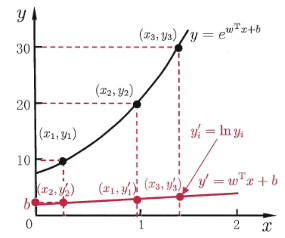
\includegraphics[width=0.309\textwidth]{pic/ML3/对数线性回归示意图}
    \caption{对数线性回归示意图}
\end{figure}


\subsubsection{广义线性模型}
考虑单调可微函数 $g(\cdot)$, 令
\begin{align*}
    y=g^{-1}\left( \bw^\top \bx+b \right)
\end{align*}
称 $g$ 为 联系函数 (link function)

\subsection{二分类任务}
预测值与输出标记
\begin{align*}
    z&=\bw^\top \bx +b \\
    y&\in \{ 0,1 \}
\end{align*}
寻找函数将分类标记与线性回归模型输出联系起来. 

最理想的函数 --- 单位阶跃函数
\begin{align*}
    y=\left\{ \begin{array}{ll}
        0 & z<0\\
        0.5 & z=0\\
        1 & z>0
    \end{array} \right.
\end{align*}
但其不连续

\begin{figure}[!htb]
    \centering
    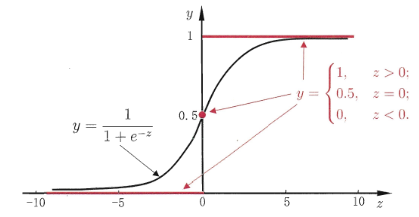
\includegraphics[width=0.42\textwidth]{pic/ML3/单 位 阶 跃 函 数 与 对 数 几 率 函 数}
    \caption{单 位 阶 跃 函 数 与 对 数 几 率 函 数}
\end{figure}

\subsubsection{对数几率回归}


\paragraph{对数几率函数(logistic function)} 于是使用对数几率函数替代. 
\begin{align*}
    y&=\frac{1}{1+e^{-z}}\\
    y&=\frac{1}{1+e^{-(\bw^\top\bx+b)}}\\
    \ln\frac{y}{1-y}&=\bw^\top\bx+b
\end{align*}


\begin{definition}[对数几率(log odds)]
    若 将 $y$ 视为样 本 $\bx$ 作为正例的可能性, 则 $1 - y$ 是其反例可能性, 两者的比值称 为 ``几 率 ''(odds), 反 映 了 $\bx$作为正例的相对可能性. 对几率取对数则得到 ``对数几率''(log odds,亦 称 logit)
    \begin{align*}
        \ln\frac{y}{1-y}
    \end{align*}
\end{definition}

优势:
\begin{enumerate}
    \item 无需假设数据分布
    \item 可得``类别''的近似概率预测
    \item 可直接应用现有数值优化算法求最优解
\end{enumerate}

\paragraph{极大似然法}来估计 $\bw$ 与 $b$. 

若将 $y$ 视为类后验概率估计 $p(y = 1 | \bx)$, 有 
\begin{align*}
    \ln\frac{p(y = 1 | \bx)}{p(y = 0 | \bx)}&=\bw^\top \bx+b\\
    p(y = 1 | \bx)&=\frac{e^{(\bw^\top\bx+b)}}{1+e^{(\bw^\top\bx+b)}}\\
    p(y = 0 | \bx)&=\frac{1}{1+e^{(\bw^\top\bx+b)}}\\
\end{align*}

给定数据集 $\{ (\bx_i, y_i) \}_{i=1}^m$, 最大化对数似然函数
\begin{align*}
    \ell(\bw,b)=\sum_{i=1}^m\ln p(y_i|\bx_i;\bw_i,b)
\end{align*}
令 $\bm\beta=(\bw;b),\hat{\bx}=(\bx,1)$, $\bw^\top\bx+b=\bm{\beta}^\top\hat{\bx}$
\begin{align*}
    p_1(\hat{\bx};\bm \beta)&=p(y=1|\hat{\bx};\bm\beta)\\
    p_0(\hat{\bx};\bm \beta)&=p(y=0|\hat{\bx};\bm\beta)=1-p_1(\hat{\bx};\bm \beta)\\
    p(y_i|\bx_i;\bw,b)&=y_ip_1(\hat{\bx};\bm \beta)+(1-y_i)p_0(\hat{\bx};\bm \beta)
\end{align*}
因为 $y_i=0,1$, 有
\begin{align*}
    \ell(\bm\beta)&=\left\{ \begin{array}{ll}
        \bm{\beta}^\top \hat{\bx}_i-\ln\left( 1+e^{\bm{\beta}^\top\hat{\bx}_i} \right)& y_i=1\\
        -\ln\left( 1+e^{\bm{\beta}^\top\hat{\bx}_i} \right) & y_i=0
    \end{array} \right.\\
    &=\sum_{i=1}^m\left( y_i\bm{\beta}^\top \hat{\bx}_i-\ln\left( 1+e^{\bm{\beta}^\top\hat{\bx}_i} \right) \right)
\end{align*}
关 于 $\bm\beta$ 的 高 阶 可 导 连 续 凸 函 数, 可以使用经 典 的 数 值 优 化 算 法  求解得
\begin{align*}
    \bm\beta^*=\argmin_{\bm\beta}-\ell(\bm\beta)
\end{align*}

\paragraph{对数几率回归总结}
主要思想:
\begin{itemize}
    \item 引入 sigmod, 关联了离散标记与线性模型
    \item sigmod 光滑, 高阶可导, 接近离散标记
    \item 得到类别接近概率似然估计
    \item 构建极大似然目标函数
    \item 优化求解: 梯度下降, 牛顿法等
\end{itemize}


\subsubsection{线性判别分析(LDA)}
(Linear Discriminant Analysis)LDA 视为一种监督降维技术. 

\begin{figure}[!htb]
    \centering
    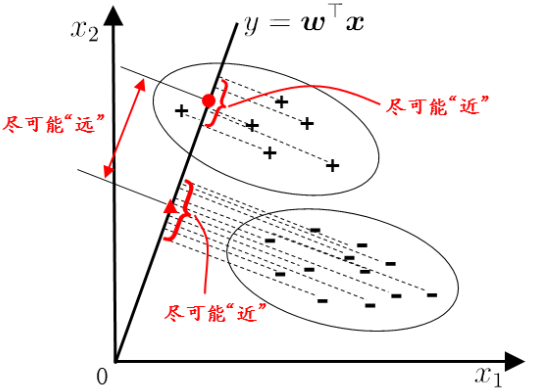
\includegraphics[width=0.42\textwidth]{pic/ML3/LDA.png}
    \caption{LDA 的 二 维 示 意 图}
\end{figure}
给定训练样例集, 设法将样例投影到一条直线上, 使得同类样例的投影点尽可能接近、异类样例的投影点尽可能远离. 

相关变量:
\begin{itemize}
    \item $\bw$: 目标直线
    \item $X_i$: 第 $i$ 类示例的集合
    \item $\bm{\mu}_i$: 第 $i$ 类示例的均值向量
    \item $\Sigma_i$: 第 $i$ 类示例的协方差矩阵
    \begin{align*}
        \Sigma_i=\sum_{\bx\in X_i}(\bx-\bm{\mu}_i)(\bx-\bm{\mu}_i)^\top
    \end{align*}
    \item $\bw^\top\bm{\mu}_0$, $\bw^\top\bm{\mu}_1$: 两类样本中心在直线上的投影.
    \item $\bw^\top\Sigma_0\bw$, $\bw^\top\Sigma_1\bw$: 两类样本的协方差
\end{itemize}

最大化目标:
\begin{align*}
    J&=\frac{\norm{\bw^\top\bm{\mu}_0-\bw^\top\bm{\mu}_1}_2^2}{\bw^\top\Sigma_0\bw+\bw^\top\Sigma_1\bw}\\
    &=\frac{\bw^\top(\bm{\mu}_0-\bm{\mu}_1)(\bm{\mu}_0-\bm{\mu}_1)^\top\bw}{\bw^\top(\Sigma_0+\Sigma_1)\bw}
\end{align*}

定义类内散度矩阵 与 类间散度矩阵:
\begin{align*}
    S_w&=\Sigma_0+\Sigma_1\\
    &=\sum_{\bx\in X_0}(\bx-\bm{\mu}_0)(\bx-\bm{\mu}_0)^\top+\sum_{\bx\in X_1}(\bx-\bm{\mu}_1)(\bx-\bm{\mu}_1)^\top\\
    S_b&=(\bm{\mu}_0-\bm{\mu}_1)(\bm{\mu}_0-\bm{\mu}_1)^\top
\end{align*}


于是最大化目标可重写为 $S_b$ 与 $S_w$ 的广义瑞利商 (generalized Rayleigh quotient)
\begin{align*}
    J=\frac{\bw^\top S_b \bw}{\bw^\top S_w \bw}
\end{align*}

令 $\bm w ^T \bm S_w \bm w=1$ 最大化上式等价形式为
\begin{align*}
    &\min_{\bw} -\bw^\top S_b \bw\\
    \st & \bw^\top S_w \bw=1
\end{align*}

运用拉格朗日乘子法
\begin{align*}
    S_b\bw=\lambda S_w\bw
\end{align*}

\paragraph{拉格朗日乘子法}
用了个对偶问题, 略过过程, 最后有
\begin{align*}
    \bw=S_w^{-1}(\bm{\mu}_0-\bm{\mu}_1)
\end{align*}
使用奇异值分解求解, i.e. $S_w=U\Sigma V^\top$, 然后得到 $S_w^{-1}=V\Sigma^{-1}U^\top$.

LDA 也可以用贝叶斯决策论解释. 

\paragraph{LDA推广---多分类任务}假定存在 $N$ 个类, 且第 $i$ 类示例数位 $m_i$.

定义全局散度矩阵
\begin{align*}
    S_t&=S_b+S_w\\
    &=\sum_{i=1}^m (\bx_i-\bm\mu)(\bx_i-\bm\mu)^\top
\end{align*}
其中 $\bm\mu$ 是所有示例的均值向量. 

再重定义类内散度矩阵, 类间散度矩阵
\begin{align*}
    S_w&=\sum_{i=1}^N S_{w_i}\\
    &=\sum_{i=1}^N \left( \sum_{\bx\in X_i}(\bx-\bm{\mu}_i)(\bx-\bm{\mu}_i)^\top \right)\\
    S_b&=S_t-S_w\\
    &=\sum_{i=1}^N m_i(\bm{\mu}_i-\bm\mu)(\bm{\mu}_i-\bm\mu)^\top
\end{align*}

使用 $S_b, S_w, S_t$ 三者中的任何两个即可, 常见的是采用优化目标
\begin{align*}
    \max_W\frac{tr(W^\top S_b W)}{W^\top S_w W}
\end{align*}
其中 $W\in\R^{d\times(N-1)}$, 通过如下广义特征值问题求解
\begin{align*}
    S_bW=\lambda S_w W
\end{align*}
$W$ 的 闭 式 解 则 是 $S_w^{-1}S_b$ 的 $N - 1$ 个最大广义特征值所对应的特征向量组成的矩阵.

多 分 类 LDA 将 样本投影到 $N - 1$ 维空间, $N - 1$ 通常远小于数据原有的属性数, 因此LDA 也常被视为一种经典的监督降维技术.

% \paragraph{LDA总结}


\subsection{多分类任务}
常用技巧: 利用二分类学习器解决多分类问题. 

\subsubsection{一对一}

\subsubsection{一对其余}

\subsubsection{比较一对一与一对其余}

\subsubsection{多对多}
Many vs Many (MvM): 若干类为正类, 若干类为反类. 

\paragraph{纠错输出码} (Error Correcting Output Code, ECOC)

\begin{figure}[!htb]
    \centering
    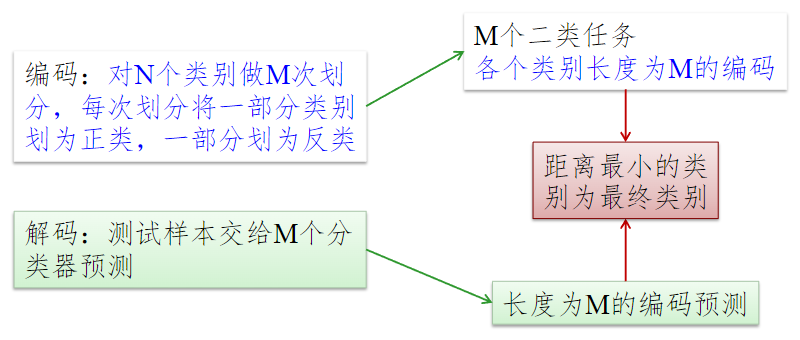
\includegraphics[width=0.42\textwidth]{pic/ML3/ECOC}
    \caption{ECOC}
\end{figure}



\subsection{类别不平衡任务}

